\documentclass[a4paper,10pt]{article}

\usepackage[utf8]{inputenc}
%\usepackage[T1]{fontenc}
%\usepackage[french]{babel}
\usepackage[margin=1in]{geometry} 
\usepackage{amsmath,amsthm,amssymb}
\usepackage{lmodern}
\usepackage{graphicx}
\usepackage{mathtools}
\usepackage{tcolorbox}
\usepackage{listings}
\newcommand{\R}{\mathbb{R}}  
\newcommand{\Z}{\mathbb{Z}}
\newcommand{\N}{\mathbb{N}}
\newcommand{\Q}{\mathbb{Q}}
\newcommand{\C}{\mathbb{C}}
%opening
\title{Intership - Sparse Coding}
\author{Thomas Rolland}
\date{}%Remove date

\begin{document}

\maketitle

\begin{abstract}
Little document to summarize sparse coding. Mainly based on the Hugo Larochelle courses.\\
\begin{center}

\textbf{This document is a draft }
 
\end{center}
\end{abstract}
\tableofcontents
%\section{Pré-requis}
%\subsection{Representation learning}
%La Representation learning ou feature learning sont des méthodes qui permettent à un système
\section{Sparse coding}
\subsection{Introduction}
\paragraph{Idea} Sparse dictionary learning is a representation learning method which aims at finding a sparse representation of the input data (in form of a linear combination of basic elements (called Atoms). The idea of using learned dictionary instead of a predefined one is based on wavelets. Thie sparse learned models has recently led to state-of-the-art result for denoising, classification,...
%UNSPERVISED LEARNING=========================================================+
\paragraph{Unsupervised learning} Only use the inputs $x^{(t)}$ ( $X = [x_1,....,x_n]$ in $\R^{m \times n}$) for learning. Automatically extract meaningful features of our data, leverage the availability of unlabeled data and add a data-dependent regularize to trainings.\\

Sparse coding is one of the neural networks used for unsupervised learning  (like restricted boltzmann machines and autoencoders).\\
The idea behind sparse coding is: For each $x^{t}$ find a latent representation $h^{t}$ such that:
\begin{itemize}
 \item[$\bullet$] It is sparese: the vector $h^{t}$ has many zeros (only few nonzero elements)
 \item[$\bullet$] We can reconstruct the original input $x^{(t)}$ as well as possible.
\end{itemize}
That mean, more formally:\\

%Formulation du problème=============================
\begin{center}
 $\min\limits_{D} \frac{1}{T} \sum_{t=1}^{T}  \min\limits_{h^{(t)}} \frac{1}{2} \| x^{(t)} - D \hspace{3px} h^{(t)} \|_2^2 + \lambda \|h^{(t)} \|_1$\\
\end{center}

 %Explicaiton de la formulation=========================
 \begin{itemize}
 \item[$\bullet$] D is a matrix of weights, usually refer to that matrix as a dictionary matrix (containt atoms) with $D \in  \R^{m \times k}$ ( k the number of atoms)
  \item[$\bullet$] $\| x^{(t)} - D \hspace{3px} h^{(t)} \|_2^2 $ is the reconstruction error
  \item[$\bullet$]$ D \hspace{3px} h^{(t)}$ is the reconstruction of $\hat{x}^{(t)}$
  \item[$\bullet$]$\|h^{(t)} \|_1$ is the sparsity penalty (more 0 in h we have, better it is)
 \end{itemize}
This two objectives fight each other. But it still a optimization problem (cf min), and we'll try to optimize it for each training example $x^{(t)}$. This is why we have a sum over all the training examples.
\newline

%Contraintes sur D======================================
\indent We also constrain the columns of D to be of norm 1 (otherwise, D could grow big while $h^{(t)}$ becomes small to satisfy the prior). And sometimes the columns are constrained to be no greather than 1.\\

However, $h^{(t)}$ is now a complicated function of $x^{(t)}$:\\
Encoder is the minimization $h(x^{(t)}) = arg\min\limits_{h^{(t)}}= \frac{1}{2} \| x^{(t)} - D \hspace{3px} h^{(t)} \|_2^2 + \lambda \|h^{(t)} \|_1$, so the optimization problem is more complicated than a simple non linear problem.\\
The idea to solve this minimization problem is \cite{NIPS2006_2979} :

\begin{lstlisting}[language=Python,frame=single]
while D not_converged :
    Fix D
    Minimize h           (1)
    Fix h 
    Minimize D           (2)
\end{lstlisting}


%DICTIONARY==================================================================+  
\paragraph{Dictionary}
We can also write $\hat{x}^{(t)} = D\hspace{3px} h(x^{(t)}) \displaystyle\sum_{\substack{k s.t.\\ h(x^{(t)})_k\neq 0}}  D.,_k h(x^{(t)} )_k$
\begin{figure}[h]
 \centering
 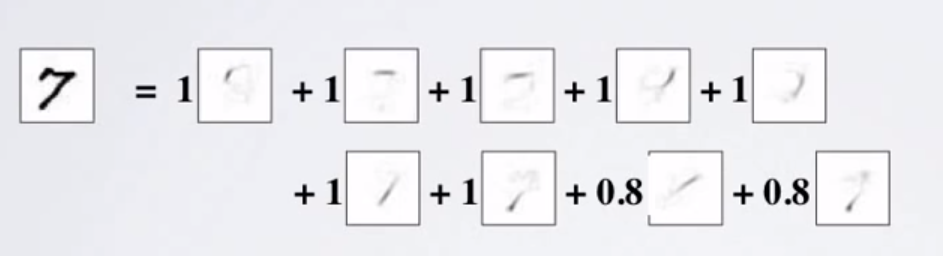
\includegraphics[scale=0.5]{spacecoding_1.png}
 % spacecoding_1.png: 943x256 px, 96dpi, 24.95x6.77 cm, bb=0 0 707 192
  \caption{Example of reconstruction using sparse coding}
\end{figure}

The images refer to $D.,_k$ (columns of D wich are not equals to 0) and the factor (1 or 0.8 in this case) refer to $h(x^{(t)} )_k$
\\We also refer to D as the dictionary:
\begin{itemize}
 \item[$\bullet$]in certain applications, we know what dictionary matrix to use
 \item[$\bullet$]often however, we have to learn it
\end{itemize}

In general we have $k<<n$ . But we can use an overcomplete dictionary with $k > m$.
\subsection{Inderence of Sparse code}
\subsubsection{Compute h}
%Inderence of sparse code=============================================
\paragraph{Idea}
Here we develop the (1) computation  from the initial idea.\\
Assume we are given a dictionary matrix D, how do we compute $h(x^{(t)})$. We have to optimize:
\begin{center}
$l(x^{(t)}) = \frac{1}{2} \| x^{t}- D h^{(t)} \|^{2}_{2} + \lambda \|h^{(t)}\|_1 w.r.t. h^{(t)}$\\ 
\end{center}
We could use a gradient descent method:\\
\begin{center}
$\Delta_{h^{(t)}} l(x^{(t)}) = D^T (D h^{(t)} - x^{(t)}) + \lambda sign(h^{(t)})$
\end{center}
The issue is L1 norm is not differentiable at 0. The solution is : if $h^(t)$ changes sign because of L1 norm gradient then clamp to 0.That mean :

$h^{(t)}_k = h^{(t)}_k   - \alpha (D_{., k})^T (D h^{(t)} - x^{(t)})$\\
\indent if  sign($h^{(t)}_k) \neq$ sign$(h^{(t)}_k - \alpha \lambda$ sign$(h^{(t)}_k) )$ then: $h^{(t)}_k = 0$\\
\indent else $h^{(t)}_k = h^{(t)}_k - \alpha \lambda$ sign$(h^{(t)}_k)$
\paragraph{ISTA (iterative Shrinkage and Thresholding Algorithm}
:
\begin{lstlisting}[language=Python,frame=single]
initialize h 
while h not_converged:
    for each h_k in h:
        h_k = h_k -alpha * transpose(D[:,k]) * (D*h - x)
        h_k = shrink(h_k,alpha*lambda_coef)
return h
\end{lstlisting}
Here \textbf{shrink(a,b) }= [..., sign$(a_i)$ max($|a_i| - b_i$, 0), ...]\\

\subsubsection{Compute D}
There are three algorithms used for  dictionary update.
\paragraph{Algorithm 1: A gradient descent method}
Our original problem is:
\begin{center}
 $\min\limits_{D} \frac{1}{T} \sum_{t=1}^{T}  \min\limits_{h^{(t)}} \frac{1}{2} \| x^{(t)} - D \hspace{3px} h^{(t)} \|_2^2 + \lambda \|h^{(t)} \|_1$\\
\end{center}
But here we assume $h(x^{(t)})$ doesn't depend on D. So we must minimize:
\begin{center}
 $\min\limits_{D} \frac{1}{T} \sum_{t=1}^{T}  \min\limits_{h^{(t)}} \frac{1}{2} \| x^{(t)} - D \hspace{3px} h^{(t)} \|_2^2 $\\
\end{center}
\begin{lstlisting}[language=Python,frame=single]
while D not_converged:
    # Perform gradient update of D
    D = D - alpha * (1/T)* sum((x - D h)* tranpose(h))
    # Renormalize the columns of D
    for each column D[:,j]:
        D[:,j] = (D[:,j] / norm(D[:,j]))

return D
\end{lstlisting}

\paragraph{Algorithm 2: Block-coordinate descent}
We must minimize:
\begin{center}
 $\min\limits_{D} \frac{1}{T} \sum_{t=1}^{T}  \min\limits_{h^{(t)}} \frac{1}{2} \| x^{(t)} - D \hspace{3px} h^{(t)} \|_2^2 $\\
\end{center}
The idea is to solve for each column $D_{., j}$ in cycle (that mean to optimize in one direction at time). For that we must set the gradient for $D_{., j}$ to zero.\\
We have:
\begin{center}
 $0 = \frac{1}{T}\sum_{t=1}^{T} (x^{(t)} - D h(x^{(t)}))$ $h^{(t)}_{j}$\\ \vspace{0.4cm}
 We separe $D_{.,j}$ from the rest of D:\\
 $0 = \frac{1}{T}\sum_{t=1}^{T} (x^{(t)} - (\sum_{i \neq j}D_{.,i}$ $h(x^{(t)})_i$ $ )$  $ - (D_{.,j}$ $h(x^{(t)})_j)$ ) $ h^{(t)}_{j}$\\ \vspace{0.4cm}
 Our aim is to find the value of $D_{.,j}$, we must isolate $D_{.,j}$ :\\
 $0 = \frac{1}{T} \sum_{t=1}^{T}(x^{(t)} h^{(t)}_{j} - (\sum_{i \neq j}D_{.,i}$ $h^{(t)}_i$ $h^{t}_{j} )$  $ - (D_{.,j}$ $h^{(t)2}_j))$\\ \vspace{0.2cm}
 
  $0 = (\sum_{t=1}^{T}(x^{(t)} h^{(t)}_{j} - (\sum_{i \neq j}D_{.,i}$ $h^{(t)}_i$ $h^{t}_{j} )$  $) - ( \sum_{t=1}^{T}( D_{.,j}$ $h^{(t)2}_j)))$\\ \vspace{0.2cm}
  
  $  \sum_{t=1}^{T}( D_{.,j}$ $h^{(t)2}_j) = \sum_{t=1}^{T}(x^{(t)} h^{(t)}_{j} - (\sum_{i \neq j}D_{.,i}$ $h^{(t)}_i$ $h^{t}_{j} )$  $) $\\  \vspace{0.2cm}
  
  $ D_{.,j}  \sum_{t=1}^{T} h^{(t)2}_j = \sum_{t=1}^{T}(x^{(t)} h^{(t)}_{j} - (\sum_{i \neq j}D_{.,i}$ $h^{(t)}_i$ $h^{t}_{j} )$  $) $\\ \vspace{0.2cm}
  
$ D_{.,j}  =\frac{1}{ \sum_{t=1}^{T} h^{(t)2}_j} \sum_{t=1}^{T}(x^{(t)} h^{(t)}_{j} - (\sum_{i \neq j}D_{.,i}$ $h^{(t)}_i$ $h^{t}_{j} )$  $) $\\ \vspace{0.2cm}

$ D_{.,j}  =\underbrace{\frac{1}{ \sum_{t=1}^{T} h^{(t)2}_j}}_{A_{j, j}} \underbrace{\sum_{t=1}^{T}(x^{(t)} h^{(t)}_{j})}_{B_{., j}}  - \sum_{i \neq j}D_{., i}($ $\underbrace{\sum_{t=1}^{T} h^{(t)}_i h^{t}_{j} ) }_{A_{i,j}}$\\ \vspace{0.2cm}
$D_{., j} = \frac{1}{A_{j, j}}(B_{., j} - D A_{., j} + D_{., j}A_{j, j})$
\end{center}  
\begin{lstlisting}[language=Python,frame=single]
while D not_converged:
    # For each column D[:,j] perform updates
    for each column D[:,j]:
        D[:,j] = (1/A[j, j])*(B[:, j] - D A[:, j] + D[:, j] A[j, j])
        # Normalization
        D[:,j] = D[:,j]/norm(D[:,j])

return D
\end{lstlisting}

\paragraph{Algorithm 3:  Online learning algorithm}
For large datasets we want to update D after  visiting each $x^{(t)}$. The solution is for each $x^{(t)}$ \cite{Mairal:2009:ODL:1553374.1553463} :
\begin{itemize}
 \item[$\bullet$]  Perform inference of $h(x^{(t)})$ after visiting each $x^{(t)}$
 \item[$\bullet$]  Update running averages of the quantities required to update D: 
        \begin{itemize}
         \item B = $\beta B + (1 - \beta) x^{(t)}h(x^{(t)})^T$
         \item A = $\beta A + (1 - \beta)h(x^{(t)}) h(x^{(t)})^T$
        \end{itemize}
\item[$\bullet$] Use current value of D as " warm start" to block-coordinate descent (warm start $\iff$ With the previous value of D)
\end{itemize}
( We have to specifie $\beta$ like a learning rate $\alpha$ in the gradient descent)

\begin{lstlisting}[language=Python,frame=single]
Initialize D # Not to 0 ! (To respect the constraint we define before)
while D not_converged:
    for each x:
        Infer code h
        #Update dictionary
        A = A +  h * transpose(h)
        B = B + x * transpose(h)
        #Batch upgrade
        #A = beta * A + ( 1 - beta ) * h * transpose(h)
        #B = beta * B + ( 1 - beta ) * x * transpose(h)
        while D not_converged:
            for each column D[:,j]:
                 D[:,j] = (1/A[j,j])*(B[:,j] - D A[:,j] + D[:,j] A[j,j])
                # Normalization
                D[:,j] = D[:,j]/norm(D[:,j]) 
\end{lstlisting}
\paragraph{Optimizing the Algorithm}
In practice, it's possible to improve the convergence speed of this algorithm by using a Mini-batch extension: By drawing $\eta > 1 $ signals at each iteration instead of a single one. 
\begin{center}
  \[    \left\{
                \begin{array}{ll}
                  A_t  = \beta A_{t-1} + \sum_{i=1}^{\eta} \alpha_{t,i}\alpha_{t,i}^{T}\\
                  B_t = \beta B_{t-1} + \sum_{i=1}^{\eta}x\alpha_{t,i}^{T}\\
                \end{array}
              \right.
  \]
\end{center}

Then $\beta = \frac{\theta + 1 - \eta}{\theta +1}$, where $\theta = t \eta$ if $ t < \eta$ and $\eta^2 + t - \eta$ if $t \geq \eta$

\subsection{Other algorithms}
There are other algorithms like Efficient Shift-Invariant Dictionary learning which refers to the problem of discovering a set of latent basis vectors that capture informative \textit{local patterns} at different locations of the input sequences and not in all input sequences \cite{Zheng:2016:ESD:2939672.2939824}. But in our problem we used dictionary learning on windows of 10ms, with approach we already capture informative local patterns, we don't need to used Shift-Invariant dictionary learning.

\subsection{Application for MNIST dataset}
The MNIST database of handwritten digits, available from Yann Lecun's website. MNIST has a training set of 60,000 examples, and a test set of 10,000 examples. It is a subset of a larger set available from NIST. The digits have been size-normalized and centered in a fixed-size image.
\begin{figure}[h]
 \centering
 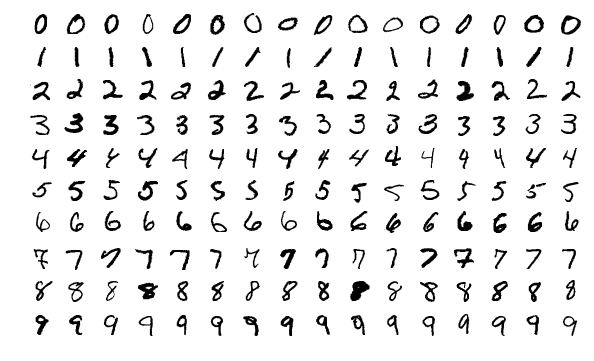
\includegraphics[scale=0.5]{MnistExamples.png}
 % MnistExamples.png: 594x361 px, 72dpi, 20.96x12.74 cm, bb=0 0 594 361
 \caption{Example of MNIST's handwitten digits}
\end{figure}
\subsubsection{Prototype}
My first task is to realise a Sparse Coding prototype to compute Sparse Coding on this dataset, using Python. The aim here, is to understand the underlying principles of this method, you can found this prototype in \texttt{Code directory} of this repository as \texttt{SparseCoding.py}. \\
There are some results of this prototype: For time saving I used only 100 digits as input.

\subsubsection{SPAMS}
SPAMS (SPArse Modeling Software) is an optimization toolbox for solving various sparse estimation problems.
\begin{itemize}
 \item Dictionary learning and matrix factorization (NMF, sparse PCA, ...)
 \item Solving sparse decomposition problems with LARS, coordinate descent, OMP, SOMP, proximal methods
 \item Solving structured sparse decomposition problems (l1/l2, l1/linf, sparse group lasso, tree-structured regularization, structured sparsity with overlapping groups,...).
\end{itemize}
It is developed and maintained by Julien Mairal (Inria), and contains sparse estimation methods resulting from collaborations with various people: notably, Francis Bach, Jean Ponce, Guillermo Sapiro, Rodolphe Jenatton and Guillaume Obozinski.\\

%====================PART 2 SPARSE CODING FOR SR=========
\section{Sparse Coding for speech recognition}
In this part of the paper we will see novel feature exraction technique based on the principles of sparse coding \cite{DL_speech_reco}. Sparse codigin deals with the problem of how represent a given audio input as a linear combination of a minimum number of basis function. The weights of the linear combination are used as feature for speech recognition (acoustic modeling). Note the input dimensionality is typically \textbf{much} less than the number of atoms in the dictionary \textit{i.e.} we use overcomplete dictionary.\\
We use Sparse Coding algorithm as describe before and we get the dictionary D and  the matrix of sparse coefficients  h.\\
\paragraph{Reflection path} In \cite{DL_speech_reco} they used spectro-temporal speech domain wich is obtained by performing a short time Fourier transform (STFT) with an analysis window of length 25 ms and a frameshit of 10 ms on the input signal. Log critical band energies are subsequently obtained by projecting the magnitude square values of the STFT output on a set of frequency weights, which are equally spaced on the Bark frequence scale, and then applying a logarithm on the output projections.
\bibliographystyle{apalike}
\bibliography{efficient-sparse-coding-algorithms.bib}

\end{document}
%KSVD
%OMP
% k doit etre deux fois trois plus grand que 8x8
